\documentclass[crop,tikz]{standalone}% 'crop' is the default for v1.0, before it was 'preview'
\usepackage{amsmath}
%\usetikzlibrary{...}% tikz package already loaded by 'tikz' option
\begin{document}
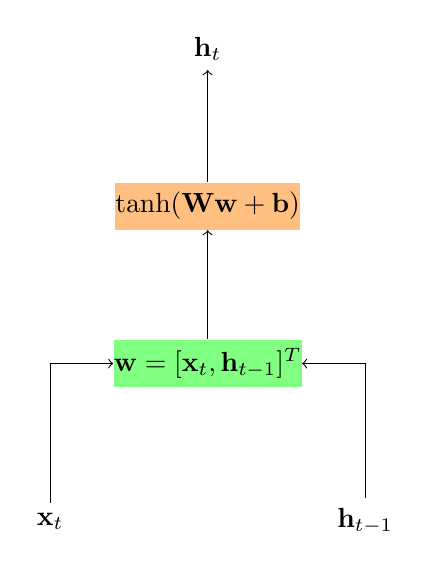
\begin{tikzpicture}
\tikzstyle{fun}=[rectangle,fill=orange!50,minimum size=17pt,inner sep=0pt]
\tikzstyle{merge}=[rectangle,fill=green!50,minimum size=17pt,inner sep=0pt]
\tikzstyle{times}=[rectangle,fill=red!50,minimum size=17pt,inner sep=0pt]
\tikzstyle{plus}=[rectangle,fill=blue!50,minimum size=17pt,inner sep=0pt]

\node (x)    at (4,0) {$\mathbf{h}_{t-1}$};
\node (hOld) at (0,0) {$\mathbf{x}_{t}$};


\node[merge] (mergeW) at (2,2) {$\mathbf{w} = [\mathbf{x}_t, \mathbf{h}_{t-1}]^T$};
\draw[->] (x) |- (mergeW);
\draw[->] (hOld) |- (mergeW);


\node[fun] (fun) at (2,4) {$\tanh(\mathbf{W} \mathbf{w} + \mathbf{b})$};
\draw[->] (mergeW) -- (fun);

\node (yNew) at (2,6) {$\mathbf{h}_{t}$};
\draw[->] (fun) -- (yNew);


\end{tikzpicture}
\end{document}